\section{Requisitos y alacance experimental}\label{sect:requisitos-alcance-experimental}
Entre los requisitos técnicos de este trabajo de fin de máster se necesita poder medir el consumo energético de un nodo y de los procesos que se estén ejecutando sobre contenedores. Para ellos, se ha seleccionado a \textit{Docker} como el gestor encargado del ciclo de vida de dichos contenedores, en base a la experiencia de uso y a su compatibilidad con el \textit{NVIDIA Container Toolkit}. Este nos proporciona un \textit{runtime}, el cual puede acceder a la GPU y hacer uso de su capacidad de cómputo.

Las cargas de trabajo sobre las que se desea poder tomar métricas de consumo consisten en procesos de codificación de video, empleando exclusivamente CPU y CPU combinada con GPU. En concreto, los codificadores que hacen uso de la GPU deben pertenecer a la generación NVENC, compatible con el \textit{NVIDIA Container Toolkit} y con las tarjetas gráficas de la marca NVIDIA.

En consecuencia, la herramienta encargada de recabar las métricas de consumo tiene que poder tomar métricas a nivel de hardware, incluyendo la GPU, y a nivel de software. Dado que la selección de la herramienta está pensada para un posterior uso en el proyecto de investigación Eco-Stream, esta debe ser capaz de desplegarse y tomar métricas sobre múltiples nodos y procesos de forma simultánea. Las métricas recolectadas deben tener un alto grado de precisión, así como de granularidad, permitiendo discernir con suficiente precisión el consumo energético del proceso respecto al consumo energético del nodo. 

Tras realizar una primera revisión de la literatura científica, en particular de los trabajos relacionados con las métricas de consumo energético en cargas de codificación de vídeo \cite{survery-videoencoding} \cite{rapl-tool} \cite{energy-rapl-mesurement}, se plantean dos hipótesis iniciales sobre los resultados esperados durante la fase de experimentación. 

La primera hipótesis afirma que los vídeos con valores elevados de SI y TI, tendrán un mayor consumo energético durante el proceso de codificación, siendo el TI la métrica con una mayor influencia sobre dicho consumo.

La segunda hipótesis se apoya en el trabajo presentado en \cite{multithread-energy-consumption-videoencoding}, donde se espera que al aumentar el número de threads y cores empleados se observe una mejora en el consumo energético y el tiempo de codificación de los códecs. Sin embargo, se plantea que esta mejora llegará a un punto de saturación a partir del cual la incorporación de recursos adicionales no proporcionará beneficios significativos. De este modo, se espera identificar el máximo número de cores que permite obtener mejoras en consumo energético y tiempo de codificación, determinando a partir de qué punto deja de ser óptimo incrementar el número de cores y threads.

%

\section{Especificación del entorno experimental}
 El sistema operativo sobre el que se han llevado a cabo las pruebas es Debian 13.1 (\texttt{amd64}, $64$ bits, x86\_64) con la versión de \textit{kernel} 6.12.90-2. Sobre este sistema se han instalado los controladores de NVIDIA en su versión 580.159.04 y el entorno CUDA en la versión 13.0. Su estabilidad y amplia compatibilidad con las herramientas software empleadas durante la fase experimental lo convierten en una opción óptima.

 Respecto al hardware sobre el que se ejecutan los experimentos, el equipo dispone de 32 GB de memoria RAM y un sistema de almacenamiento secundario HDD de 2 TB. La CPU seleccionada es una Intel i7-4790K de 8 cores; permite tomar métricas de consumo energético de prácticamente cualquier componente del sistema mediante RAPL \cite{intel-processor-sepcts}.

 La tarjeta gráfica seleccionada es una NVIDIA Quadro M4000 \cite{nvidia-quadro-m4000}, elegida entre el conjunto de GPUs disponibles en el laboratorio. En primer lugar, la tarjeta es compatible con la interfaz NVIDIA System Management (NVIDIA-SMI) \cite{nvidia-smi}, herramienta empleada para la monitorización y extracción de métricas relacionadas con el estado y el consumo energético de la tarjeta gráfica. Asimismo, ofrece soporte para las versiones de CUDA y \textit{NVIDIA Container Toolkit} \cite{nvidia-container-toolkit}, lo cual permite hacer uso de la GPU desde los contenedores y ejecutar cargas de trabajo mediante aceleración de hardware.

 Esta tarjeta gráfica incluye soporte para la tecnología NVENC, la cual permite usar los codificadores de hardware H.264 (AVC) y H.265 (HEVC) en diferentes formatos de codificación, entre los cuales aparecen referenciados en la tabla \ref{tab:nvidia-matrix-capacity}.

 \begin{table}[h!]
  \center
  \begin{tabular}{cccc}
  \hline
  \textbf{Codificador} & \textbf{Formato} & \textbf{CPU} & \textbf{GPU} \\ \hline
  H.264                & YUV 4:2:0        & x            & X            \\
  H.264                & YUV 4:4:4        & X            & X            \\
  H.264                & Lossless         & X            & X*           \\
  H.265                & 4K YUV 4:2:0     & X            & X            \\ \hline
  \end{tabular}
  \label{tab:nvidia-matrix-capacity}
  \caption{Matriz de Capacidad de Codificación de Video de NVIDIA Quadro M4000}
 \end{table}

% - Herraminetas Sofware a utilizas
 %    - ffmpeg
 %    - schapahndre
 %    - monitor
 %    - kepler
 
 Para llevar a cabo los diferentes procesos experimentales, serán necesarias diferentes aplicaciones: \textit{FFmpeg}, encargada de la transcodificación de vídeo; \textit{Docker}, encargado de la creación, despliegue y gestión de contenedores sobre los que se ejecutarán múltiples procesos; \textit{Bash}, como intérprete de comandos para automatizar la ejecución y el procesamiento de resultados de los \textit{scripts} y procesos asociados.
 
 En cuanto a las herramientas con las que se llevará a cabo la monitorización y toma de métricas de consumo energético, se ha realizado una búsqueda entre diversos repositorios, fuentes académicas y papers, como \cite{container-metrics-kubernetes}, y se ha llevado a cabo una selección de las herramientas consolidadas en el estado del arte. Estas dos herramientas han sido: \textit{Kepler} \cite{kepler} y \textit{Scaphandre} \cite{scaphandre}.
 
 Adicionalmente, también se han proporcionado dos herramientas por parte de Juan Gutiérrez Aguado, uno de los directores del proyecto Eco-Stream: \textit{EnergyMeter}, empleada como referencia de consumo energético del sistema basado en las métricas del sistema obtenidas por RAPL; Y \textit{Monitor}, una herramienta desarrollada por Juan Gutiérrez Aguado empleada como alternativa a las herramientas anteriores, la cual permite medir el consumo de una carga de trabajo desplegada sobre uno o varios contenedores de forma simultánea y muy precisa. Las capacidades y alcance de cada una de estas herramientas de medición se resumen en la tabla \ref{tab:especi-herramientas-capacidad-metricas}.
 
 Para el procesamiento e interpretación de los datos se utilizará principalmente \textit{Python}, haciendo uso de la librería \textit{Pandas} para la manipulación y almacenamiento de datos en formato CSV. Asimismo, la generación de gráficos comparativos se basará en las librerías \textit{Matplotlib} y \textit{Seaborn}. En particular, \textit{Seaborn} simplifica la representación de estructuras de datos complejas y permite obtener visualizaciones más refinadas e intuitivas.

 \begin{table}[h!]
      \centering
      \begin{tabular}{|c|c|c|c|c|}
      \hline
      \rowcolor[HTML]{C0C0C0} 
      \textit{\textbf{HERRAMIENTA}}                          & \textit{\textbf{NODO}} & \multicolumn{1}{l|}{\cellcolor[HTML]{C0C0C0}\textit{\textbf{PROCESO}}} & \multicolumn{1}{l|}{\cellcolor[HTML]{C0C0C0}\textit{\textbf{CPU}}} & \multicolumn{1}{l|}{\cellcolor[HTML]{C0C0C0}\textit{\textbf{GPU}}} \\ \hline
      \cellcolor[HTML]{EFEFEF}\textit{\textbf{Energy Meter}} & \textbf{X}             & \textbf{-}                                                             & \textbf{X}                                                         & \textbf{-}                                                         \\ \hline
      \cellcolor[HTML]{EFEFEF}\textit{\textbf{Kepler}}       & \textbf{X}             & \textbf{X}                                                             & \textbf{X}                                                         & \textbf{X}                                                         \\ \hline
      \cellcolor[HTML]{EFEFEF}\textit{\textbf{Scaphandre}}   & \textbf{X}             & \textbf{X}                                                             & \textbf{X}                                                         & \textbf{-}                                                         \\ \hline
      \cellcolor[HTML]{EFEFEF}\textit{\textbf{Monitor}}      & \textbf{X}             & \textbf{X}                                                             & \textbf{X}                                                         & \textbf{-}                                                         \\ \hline
      \end{tabular}
      \label{tab:especi-herramientas-capacidad-metricas}
      \caption{Capacidad de toma de metricas de las Herramientas}
      \end{table}

\section{Planificación y Estimación de costes}
% - Diagrama de gant
\subsection{Planificación del Desarrollo del Proyecto}
El inicio del desarrollo del proyecto, se ha fijado para la fecha del 20 Mayo, ya que esa es la fecha en la que se inicia mi actividad laboral como Personar No Doctorado Investigado(PDI). Simultaneamente, se iniciará la redacción del trabajo fin de master (TFM), sobre el cual se iran anotando los abances y decisiones tecnicas en cada uno de los apartados de la planificacion. 

El primer paso para iniciar el desarrollo del proyecto sera definir el alcance, objetivos que se desan lograr e hipotesis iniciales en base al estado del arte en el contexto de la codificacion de video y la estimacion de consumo energetico de cargas de trabajo desplegadas sobre contenedores. Una vez establecidos los requisitos y necesidades tecnicas, se inciaria la preparacion del entorno sobre el cual se desarrollaran las distintas pruebas, instalando sistema operatico y aplicaciones necesarias.

A continuacion se seleccionaran los videos empleados para llevar a cabo los experimentos de las secciones de experimentacion. Se utilizaran los videos que el servidor de contenido del proyecto Eco-Stream alberga. En concreto se  utilizaran los video del directorio \textbf{test}, los cuales proviene de CableLabs y Blender \cite{cable-labs} \cite{blender-videos}. Estos se encuentran dividiso en chunks de 2 segundo de duración que conservan todas las propiedades de calidad de cada uno de los videos originales. 

Una vez determinado el origen de los videos se definira el conjunto 

A continuacion, se seleccionarán el conjunto de videos a utilizar como bateria de puerbas y los criterios de seleccion para cada una de las fases experimentales. En este caso, dado que se requiere saber si las metricas Spatial Information(SI) y Temporal Information (TI) de los videos, afecta al consumo energetico 


\begin{figure}[h!]
    \centering
    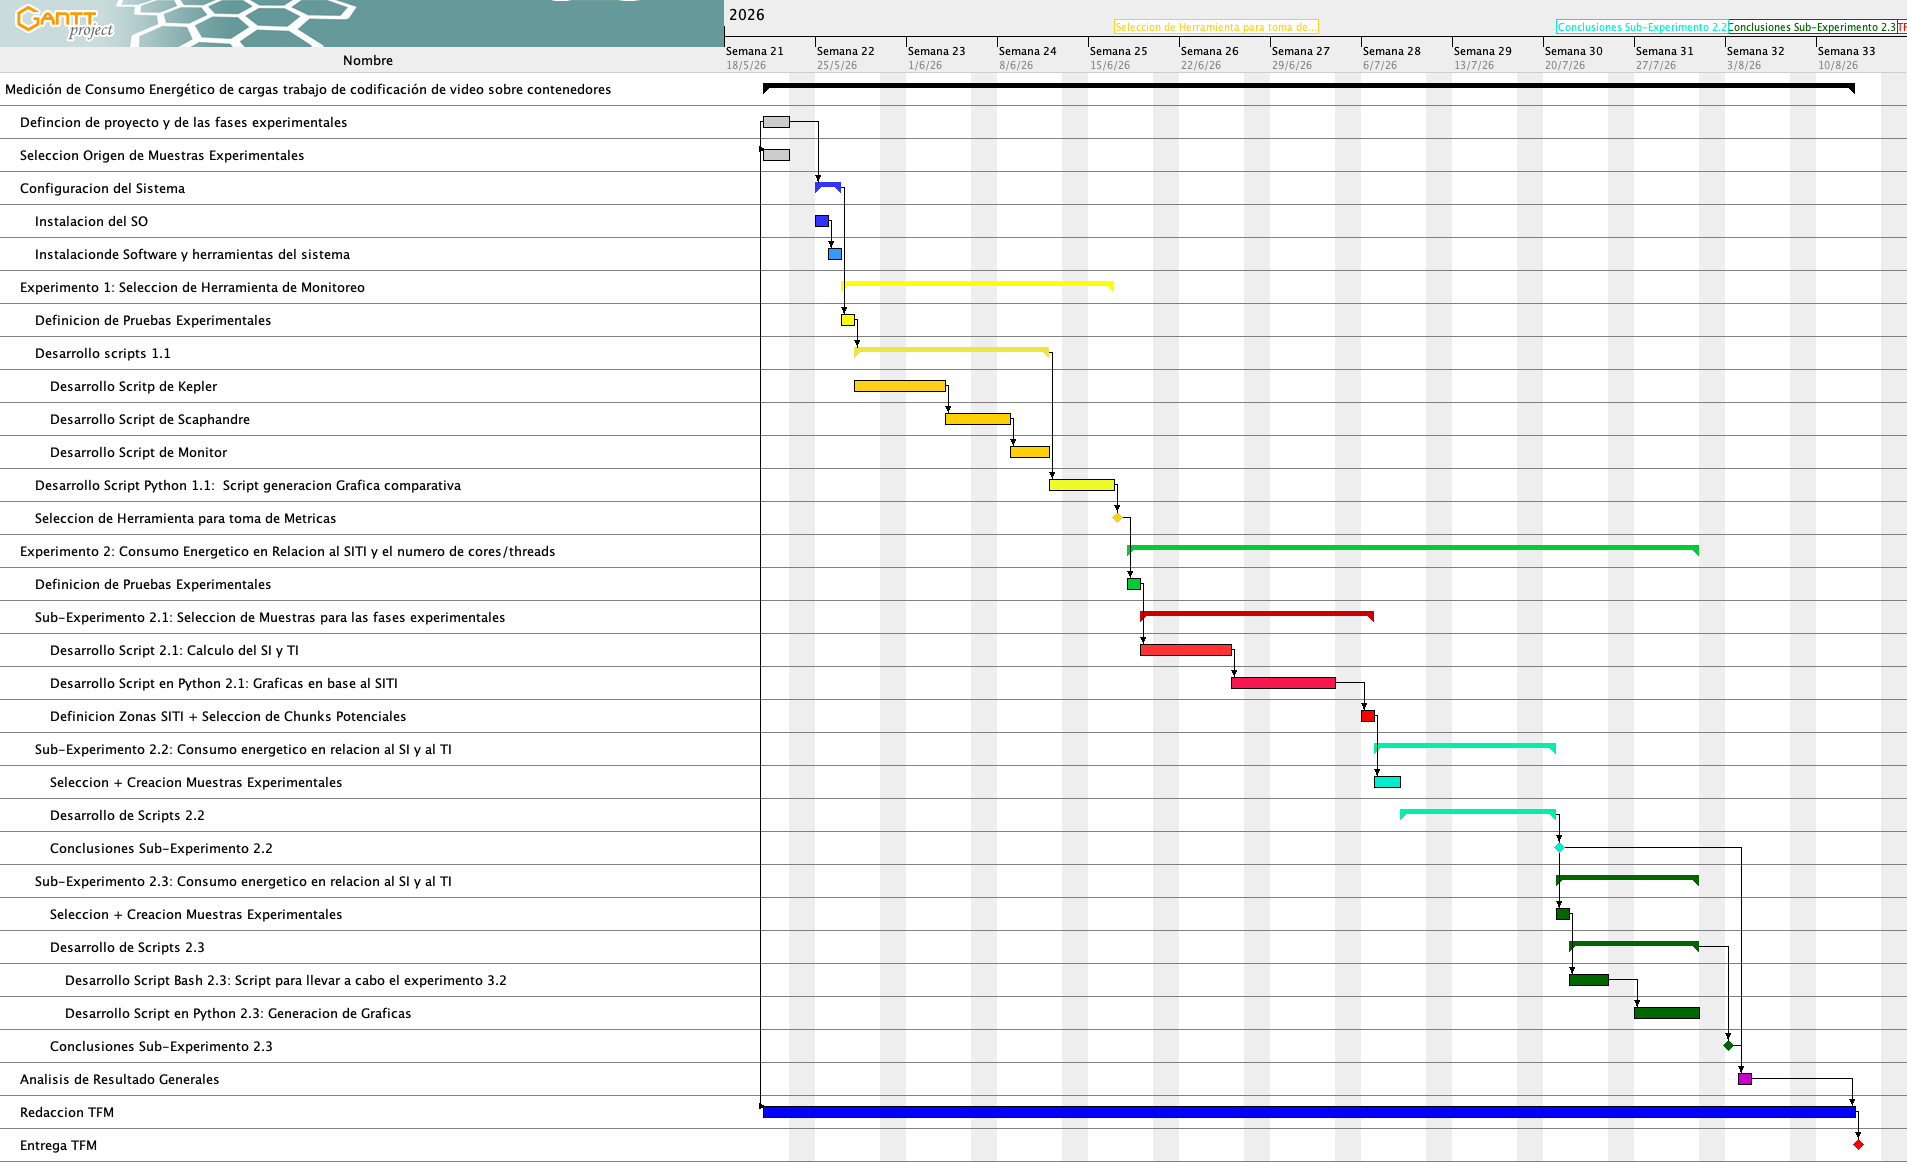
\includegraphics[width=\linewidth]{figs/PlanificacionInicial.png}
    \caption{Planificacion inicial del Desarrollo del Proyecto}
    \label{fig:expect-ganttinicial}
\end{figure}

\subsection{Estiamaciones Iniciales de Costes}
% - Excell de costes estimados




